% Performances et conclusion


\begin{frame}[c]
  \frametitle{Implementation}

\tval{Workflow}:
\begin{itemize}
  \item Read and translate the models with \tval{OCaml}\\
        \quad\f Integrated to \Pint\\
  \item Express the problem in \tval{ASP} (logic programming)\\
        \quad\f Solved with \tval{Clingo} (\tval{Gringo} + \tval{Clasp})
\end{itemize}

\bigskip
\tval{Complexity}: linear in the number of genes, exponential in the number of regulators of one gene

\pause
\bigskip
\small
\begin{tabular}{r||r@{+}l|c|c||c|c||c|c|}
\multicolumn{5}{c||}{Model specifications} & \multicolumn{2}{c||}{IG inference} & \multicolumn{2}{c|}{Parameters inference}\\
\hline
\tval{Name} & S & CS & P & A & $\Delta t$ & Edges & $\Delta t$ & Parameters\\
\hline
  \tval{\ex{egfr20}} & \tval{20} & 22 & 152 & 399 & \tval{1s} & 50 & \tval{1s} & 191\\
\hline
  \tval{\ex{tcrsig40}} & \tval{40} & 14 & 156 & 301 & \tval{1s} & 54 & \tval{1s} & 143\\
\hline
  \tval{\ex{tcrsig94}} & \tval{94} & 39 & 448 & 1124 & \tval{13s} & 169 & $\infty$ & $2.10^9$\\
\hline
  \tval{\ex{egfr104}} & \tval{104} & 89~ & 748 & 2356 & \tval{4min} & 241 & \tval{1min 30s} & $1.10^6 / 2.10^6$\\
\hline
\end{tabular}

S = Sorts \quad CS = Cooperative sorts \quad P = Processes \quad A = Actions

\cmodels
\end{frame}



\begin{frame}[c]
  \frametitle{Summary}

\begin{enumerate}[1.]
  \item Inference of the \tval{complete Interaction Graph}
  \item Inference of the \tval{possibly partial Parametrization}
  \item Enumerate all full \& \tval{admissible Parametrizations}
\end{enumerate}
\quad\quad\f Exhaustive approaches

\pause
\bigskip
\begin{flushright}
\Large
\textcolor{couleurtheme}{Conclusion}\hspace*{2.7em}
\end{flushright}

\medskip
Existing translation: René Thomas $\rightsquigarrow$ Process Hitting

\smallskip
New translation: Process Hitting $\rightsquigarrow$ René Thomas

\smallskip
\begin{fleches}
  \item New \tval{formal link} between the two models
  \item More \tval{visibility} to the Process Hitting
\end{fleches}
\end{frame}



\section[x]{Acknowledgments}

\begin{frame}[c]
  \frametitle{Joint work}

\tval{Inoue Laboratory}: National Institute of Informatics / Sokendai / Tokyo (Japan)

\smallskip
\tval{MeForBio}: IRCCyN / École Centrale de Nantes / Nantes (France)

\smallskip
\tval{BISON}: Institut für Automatik / ETH / Zürich (Switzerland)

\bigskip\bigskip\footnotesize
\begin{tabular}{cc}
  $\left.\text{\begin{tabular}{c}
    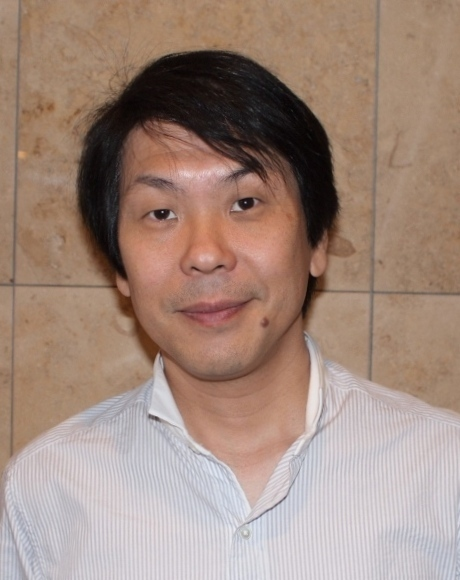
\includegraphics[height=1.5cm]{figs/Inoue-sensei.jpg} \\ \tval{Katsumi INOUE} \\ Professor \& team leader
  \end{tabular}}\right\}\text{\tval{Inoue Laboratory}}$
  &
  $\left.\text{\begin{tabular}{c}
    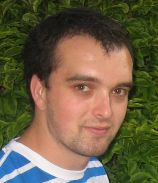
\includegraphics[height=1.5cm]{figs/Loic.jpg} \\ \tval{Loïc PAULEVÉ} \\ Post-doc
  \end{tabular}}\right\}\text{\tval{BISON}}$
  \\ & \\ & \\
  \multicolumn{2}{l}{$\left.\text{\begin{tabular}{ccc}
      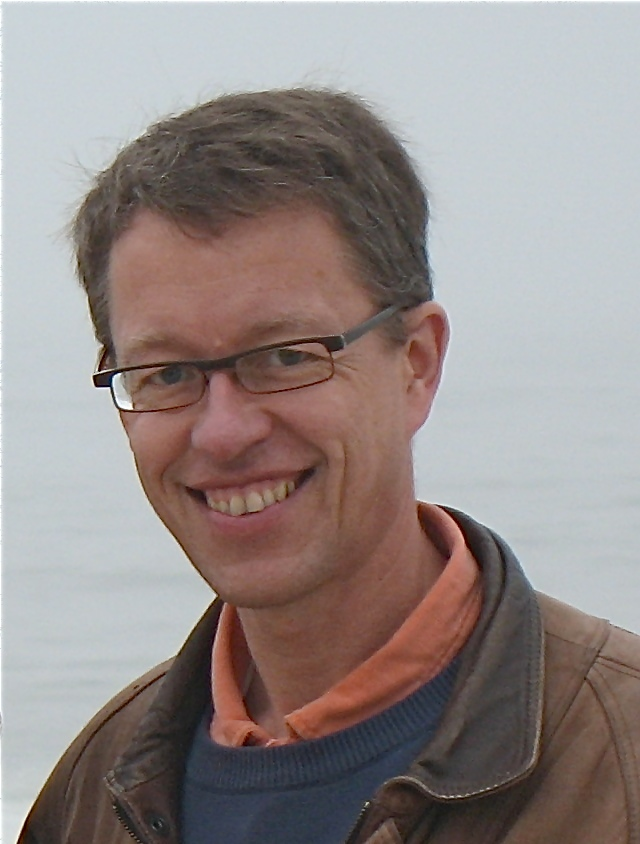
\includegraphics[height=1.5cm]{figs/Olivier.jpg}
    & 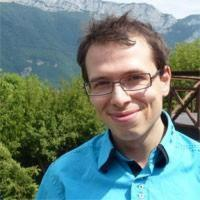
\includegraphics[height=1.5cm]{figs/Morgan.jpg}
    & 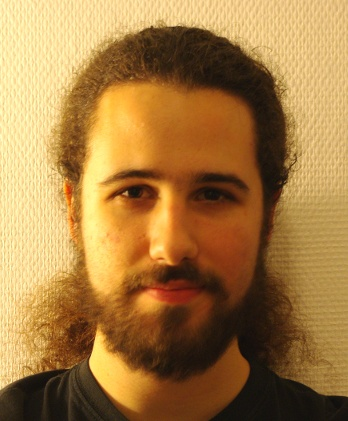
\includegraphics[height=1.5cm]{figs/Moi.jpg} \\
      \tval{Olivier ROUX} & \tval{Morgan MAGNIN} & \tval{Maxime FOLSCHETTE} \\
      Professor \& team leader & Associate professor & 2\textsuperscript{nd} year PhD student
  \end{tabular}}\right\}\text{\tval{MeForBio}}$}
\end{tabular}
\end{frame}
